\section{Results and discussion}

\subsection{Probe calibration and test liquids}\label{subsec:res-calib}
The calibration curves with the test saline solution (\qty{20}{ppt}) and methyl hydrate largely agree with the theoretical values \parencite{Nyshadham1992} (Figure~\ref{fig:calib-results}), with a \ac{rmse} of \num{1.14} and \num{0.94} respectively.
Figure~\ref{fig:calib-results} also highlights the chosen frequency ranges for remote sensing applications.

\begin{figure}[ht!]
    \centering
    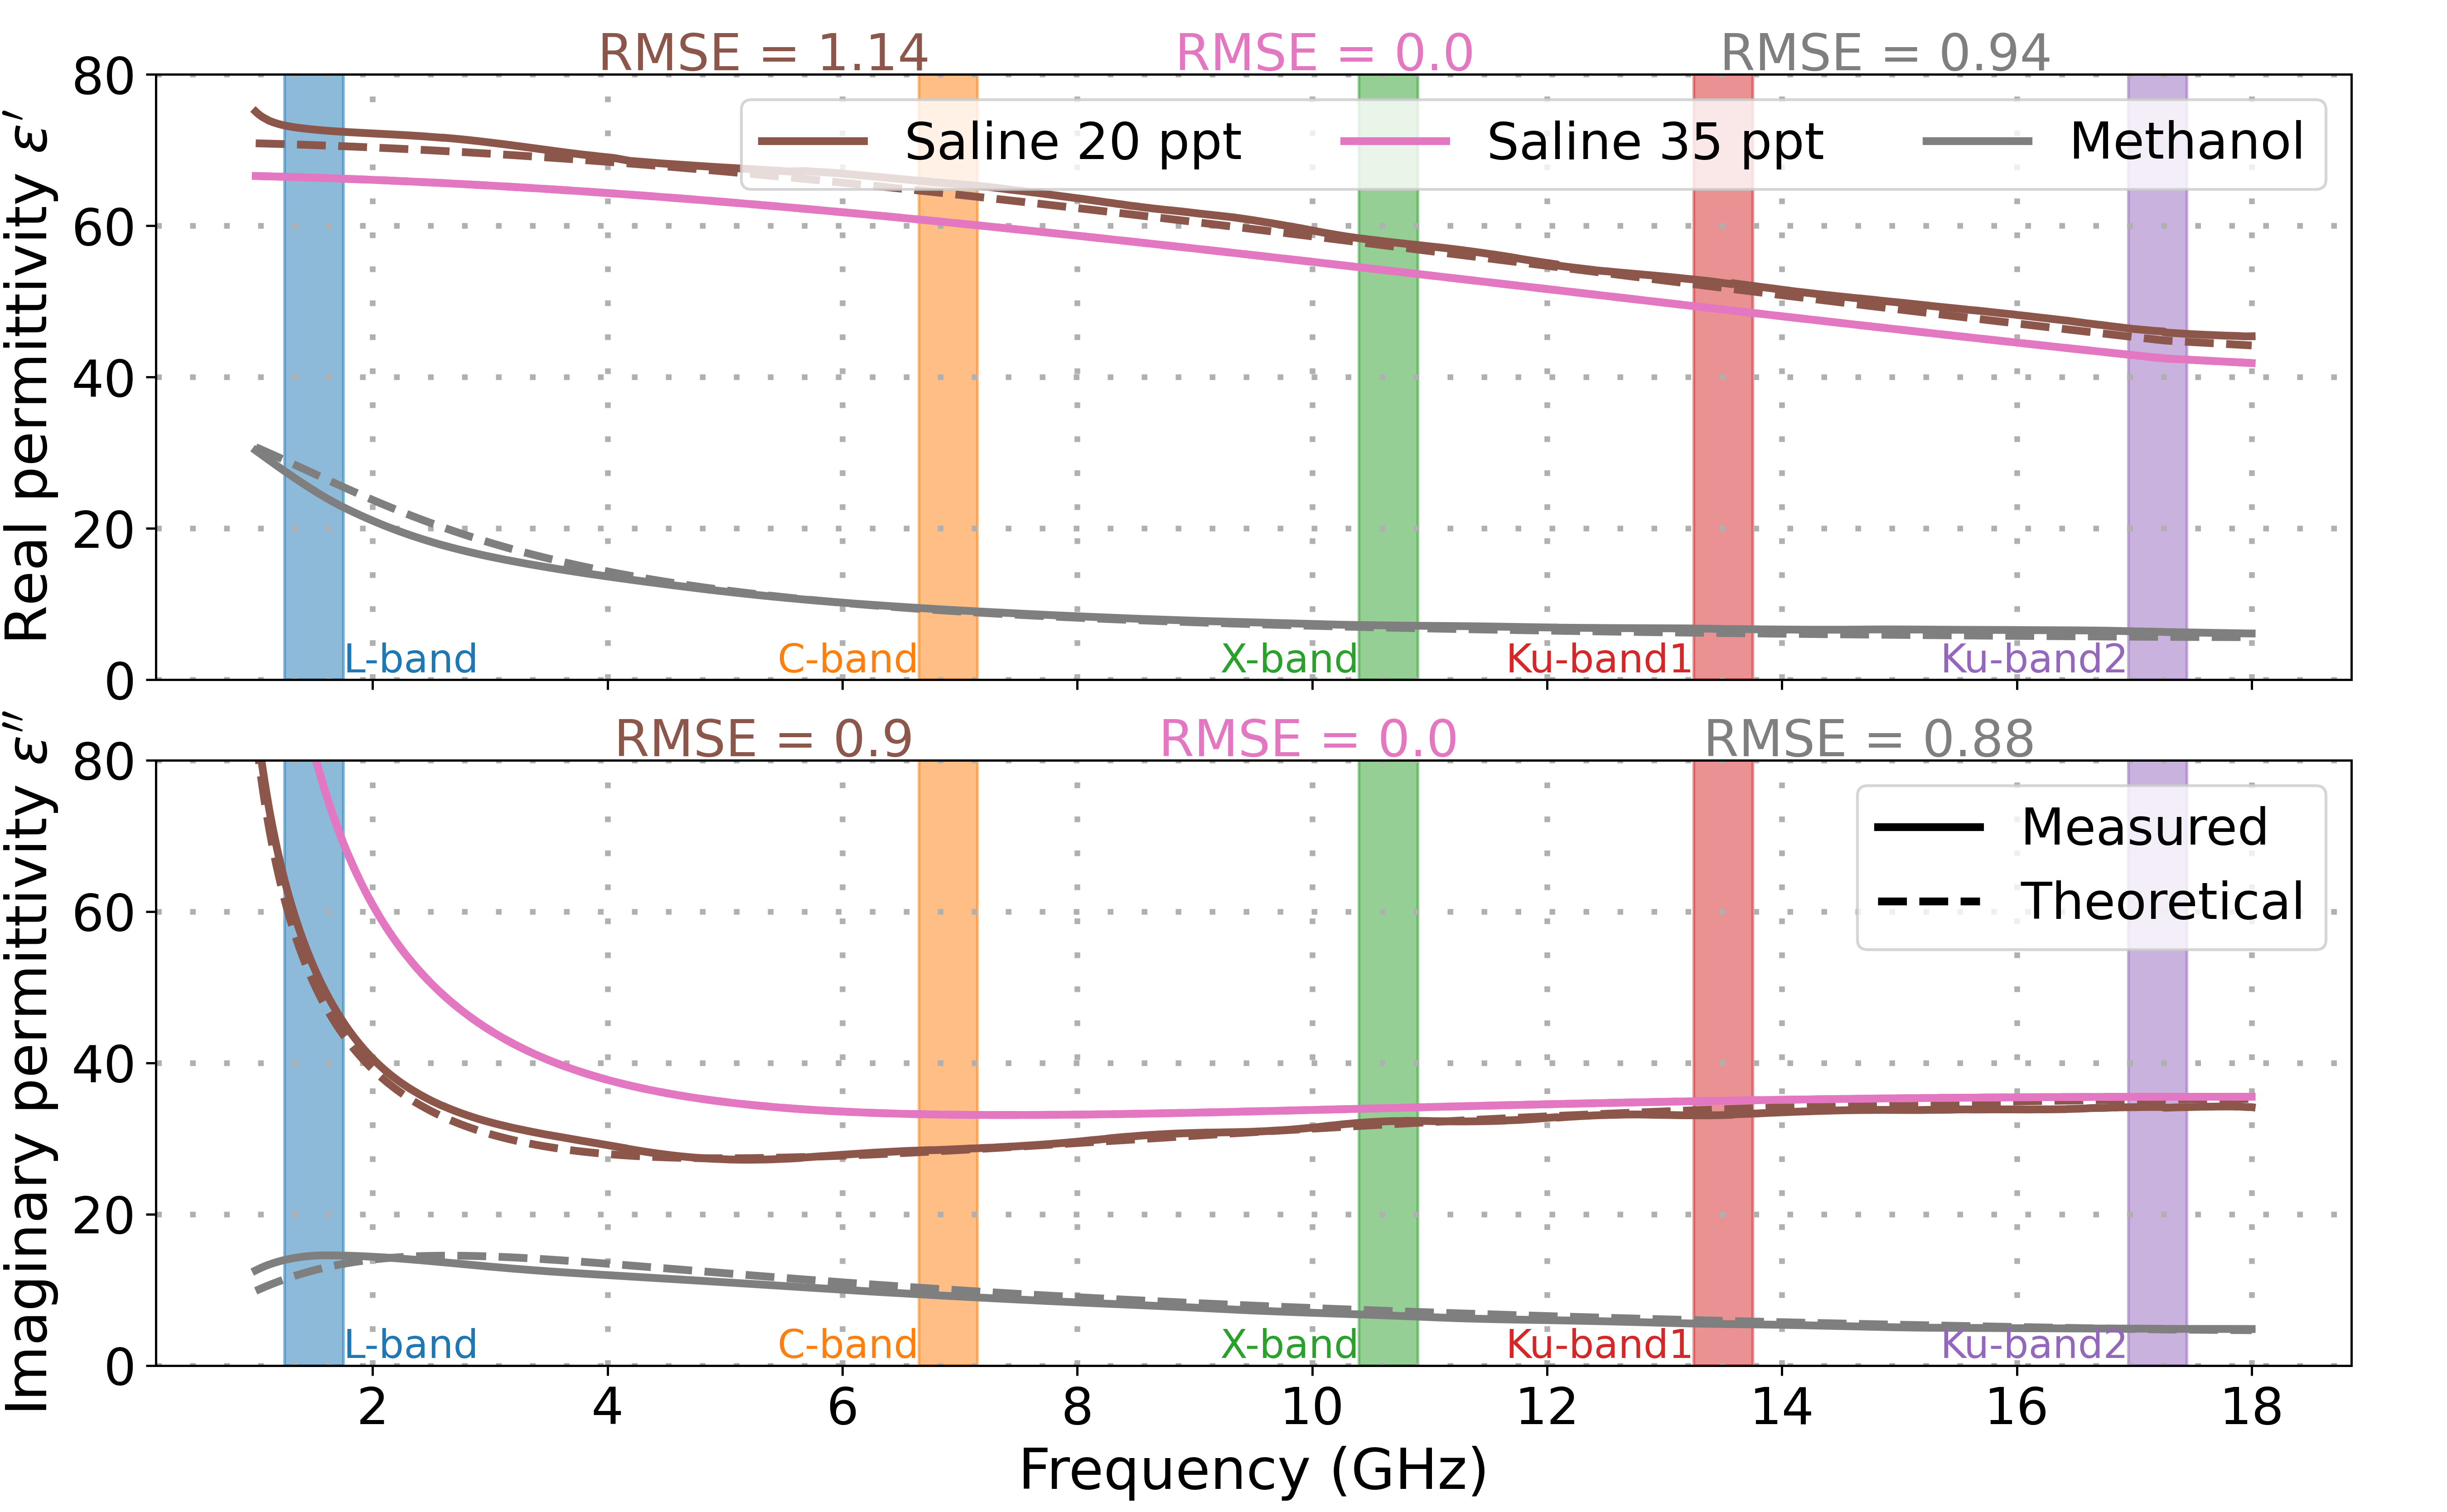
\includegraphics[width=\columnwidth]{Images/calibration-results.png}
    \caption[]{Theoretical and measured permittivity of saline solution and methanol with their associated \ac{rmse}. The selected relevant frequency ranges for remote sensing applications were also highlighted}\label{fig:calib-results}
\end{figure}

\subsection{Signal penetration depth}

\begin{figure}[ht!]
    \centering
    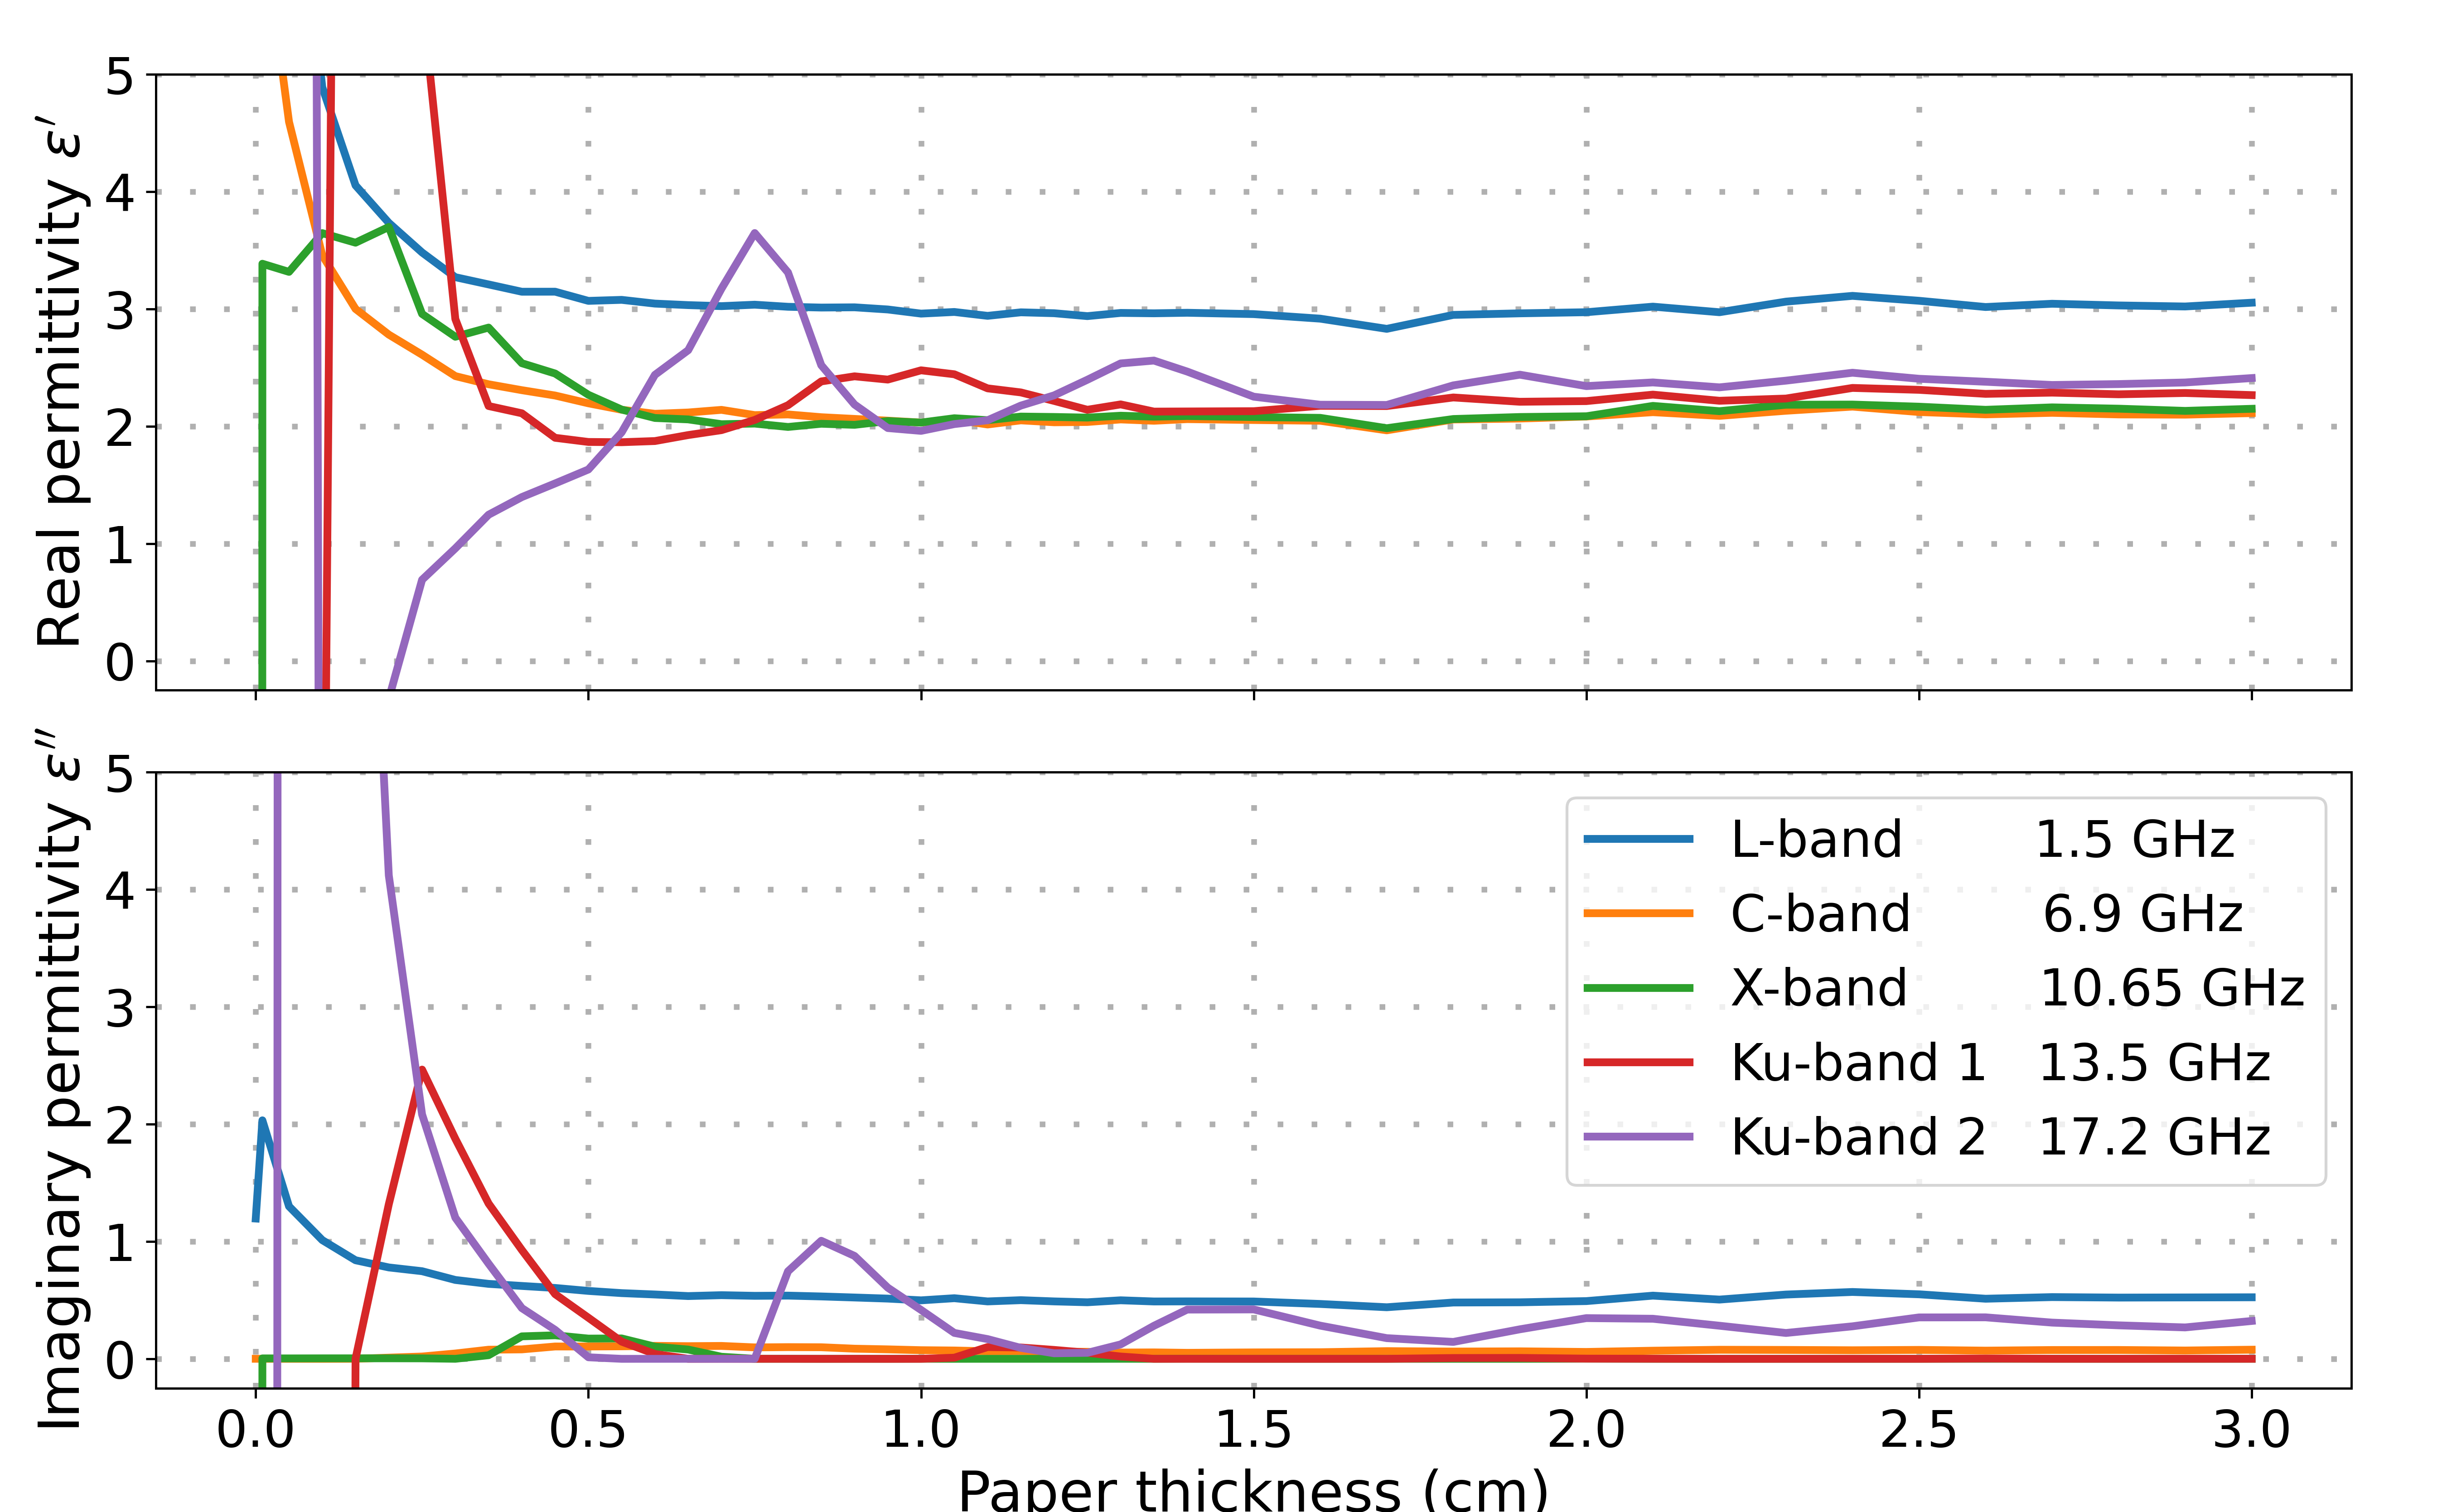
\includegraphics[width=\columnwidth]{Images/dry-paper.png}
    \caption[]{Estimation of the probe signal penetration depth on dried paper for relevant frequencies}\label{fig:dry-paper}
\end{figure}

For dry paper, at L-band (\qty{1.4}{\giga\hertz}), the curve stabilized around \qty{0.5}{\cm} for a value of \(\varepsilon^\prime = 3\) which is coherent with \parencite{Elrayes1987} who found a value around \(\varepsilon^\prime\approx2.9\) at \qty{1}{\giga\hertz}.
Figure~\ref{fig:dry-paper} also shows that the probe signal stabilizes around \qty{0.75}{\cm} for the other bands.
Considering that the outer diameter of the probe is of \qty{13.2}{\mm}, the results are consistent with the rule of thumb proposed by \textcite{Elrayes1987} that the probe penetration depth in a low loss material such as paper is approximately equal to the inside diameter of the outer conducting cylinder of the probe (see left side of figure~\ref{fig:probe-scheme}, measurement 2b = \qty{13.2}{\mm}).

% Measurements using the OECP are only based on the transient (not radiated) wave whose propagation is limited throughout the close volume of the material at the contact surface with the OECP’s aperture.
% However, slight amount of radiation waves also propagate through the material, reflect against the sample edges, then may get back to the probe, causing so measurements errors. This is the reason why the saline solution containers are chosen to be sufficiently large to allow waves damping and avoid radiation reflections.
% In thin materials, radiations are more likely to reflect into the probe. To reduce this effect, it is important to work with greater wavelengths where the probe’s radiation is neglectable. This can be achieved by using low permittivity dielectrics (like paper) and working at lower frequencies. However, at higher frequencies where the wavelength is reduced and gets closer to the OECP’s cross section, it becomes impossible to prevent radiative waves effect.
% The only allowable option is to rely on the result obtained at lower frequencies. This is justified by the fact that the obtained depth is relatively constant for all the frequencies up to the X-Band. Moreover, when the paper is wet, which causes damping, the result is the same for all the frequencies without exception. Damping has prevented radiative waves, but has also reduced the extent of the transient wave, which is why the dry paper result at low frequency is estimated to be the most reliable.
% For the measurement made during this work, the samples a sufficiently thick (more than 10cm) to avoid the radiation effect for the materials’ permittivity range.


\begin{figure}[ht!]
    \centering  
    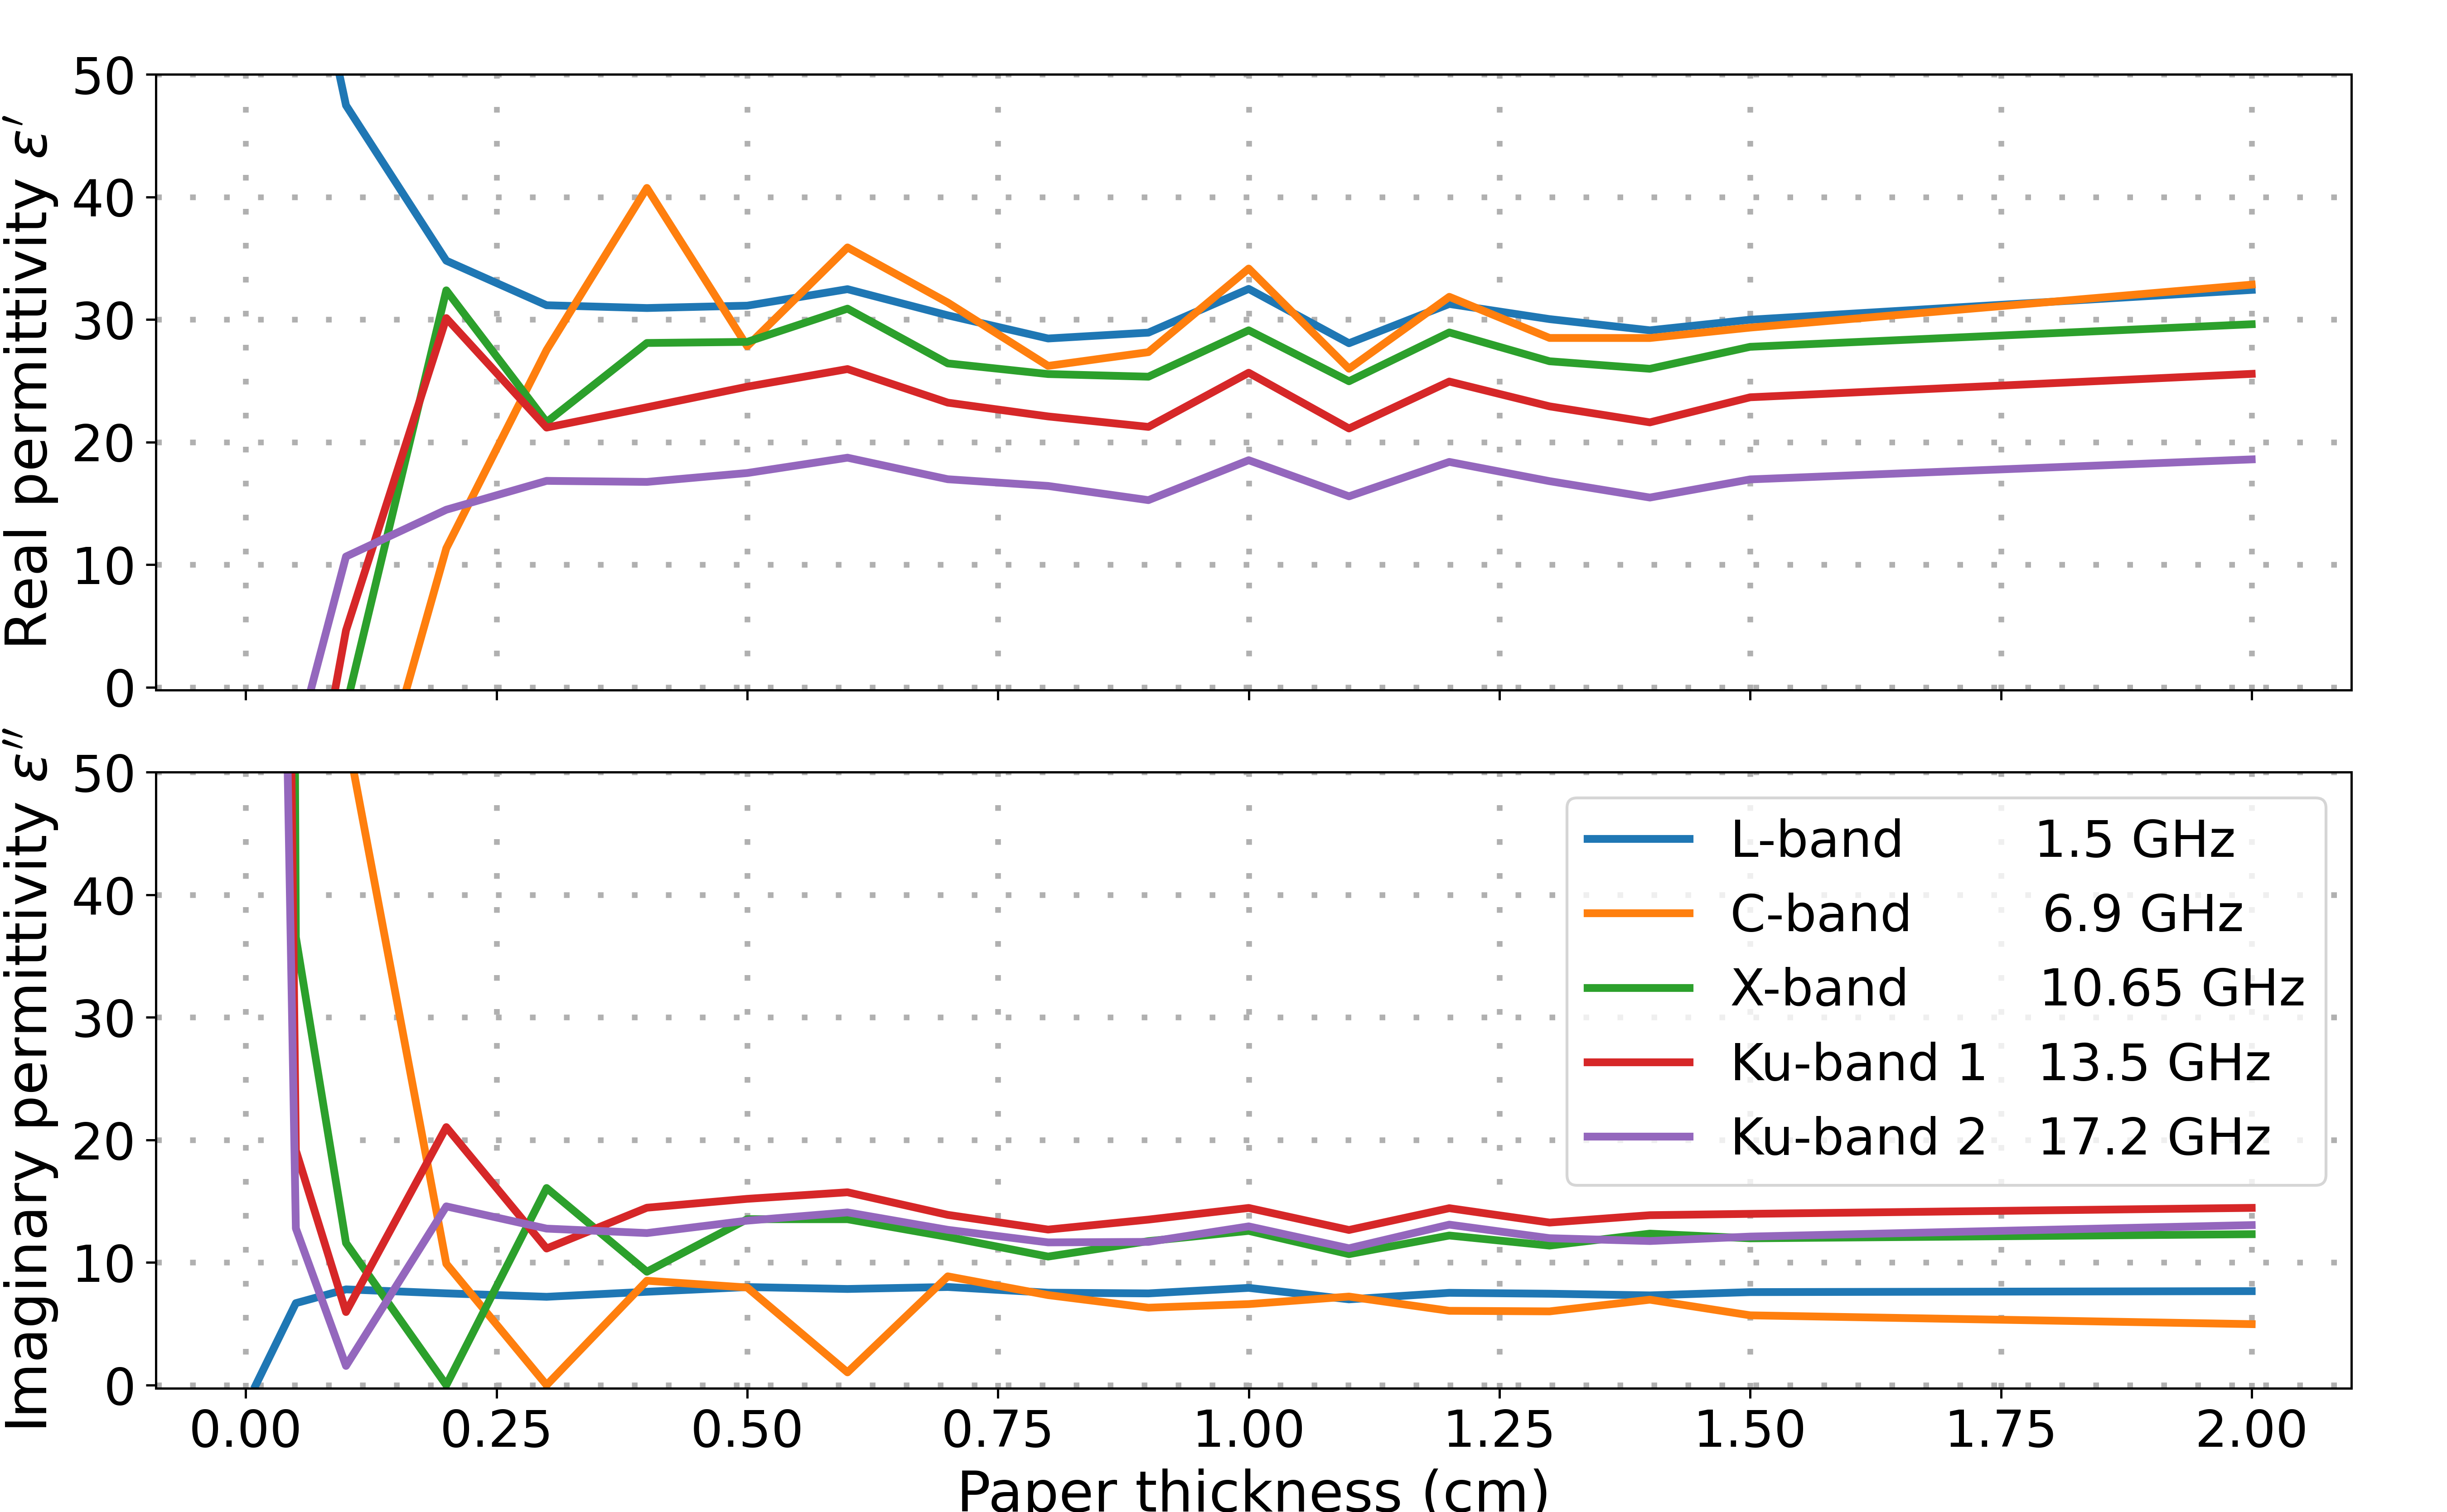
\includegraphics[width=\columnwidth]{Images/wet-paper.png}
    \caption[]{Estimation of the probe signal penetration depth on soaked paper for relevant frequencies}\label{fig:wet-paper}
\end{figure}

Figure~\ref{fig:wet-paper} results for wet paper are interpreted similarly.
However, since the paper's water content increases the dielectric loss, the real permittivity decreases for higher frequencies.
The signal loss from the conducting copper plate noticeably happens with fewer stacked sheets than with dry paper.
The probe's penetration depth in higher loss material can be estimated at around \qty{0.3}{\cm}.
Another noticeable difference between dry and wet paper comes from the oscillations with both Ku-band frequencies between \qtyrange{0.5}{1.5}{\cm} for dry paper.
These oscillations result from noise created by unwanted reflection in the dry paper medium.
Indeed, the probe signal in a medium such as dry paper at high frequencies, where the wavelengths are closer in scale to the \ac{oecp} cross-section, is more likely to be reflected on the sample edge and cause unwanted fluctuations in the reflection readings.
At frequencies closer to L-band and C-band, where the wavelengths are larger, such unwanted reflections are negligible.
In liquids such as the saline solutions used in the probe calibration process or in a moist medium such as wet paper, the probe signal is damped, preventing unwanted reflections.
This signal damping also causes the penetration depth to be equal across all frequencies in the wet medium. 
These penetration depths mean that, to safely measure only the desired sample and not its container, a safe minimal soil depth would be over \qty{2}{\cm}.
In the present study, the soil sample used are well over this limit with a \qty{10}{\cm} depth.

% See table~\ref{tab:dry-wet-paper} for a summary of the penetration depths.
% \begin{table}[ht!]
%     \centering
%     \caption{Penetration depth (cm) at different frequency in dry and wet paper sheet stacks}\label{tab:dry-wet-paper}
%     \begin{tabular}{r l c c c c}
%         Medium & L-band & C-band & X-band & Ku-band 1 & Ku-band 2 \\
%         \midrule\midrule
%         Dry paper & 0.5 & 0.75 & 0.75 & 1.25 & 1.5 \\
%         Wet paper & 0.3 & 0.3  & 0.3  & 0.3  & 0.3 \\
%     \end{tabular}
% \end{table}

% These results may seem contradictory, where usually, with constant permittivity, the penetration depth would decrease with the frequency.
% In our case, the opposite happens since water permittivity decreases with frequency

\subsection{Dry sand spectrum}
Since the dry sand permittivity does not vary in this range of temperature, its real and imaginary permittivity are compared to literature data from \textcite{Matzler1998} (see Figure~\ref{fig:dry-sand}).
In \parencite{Matzler1998}, the permittivity of dry sand gathered in the Sahara Desert in the frequency range of \qtyrange{0.245}{6}{\giga\hertz} was found to be around \(\varepsilon = 2.6 - \left[0.13, 0.012\right]j\).

\begin{figure}[ht!]
    \centering
    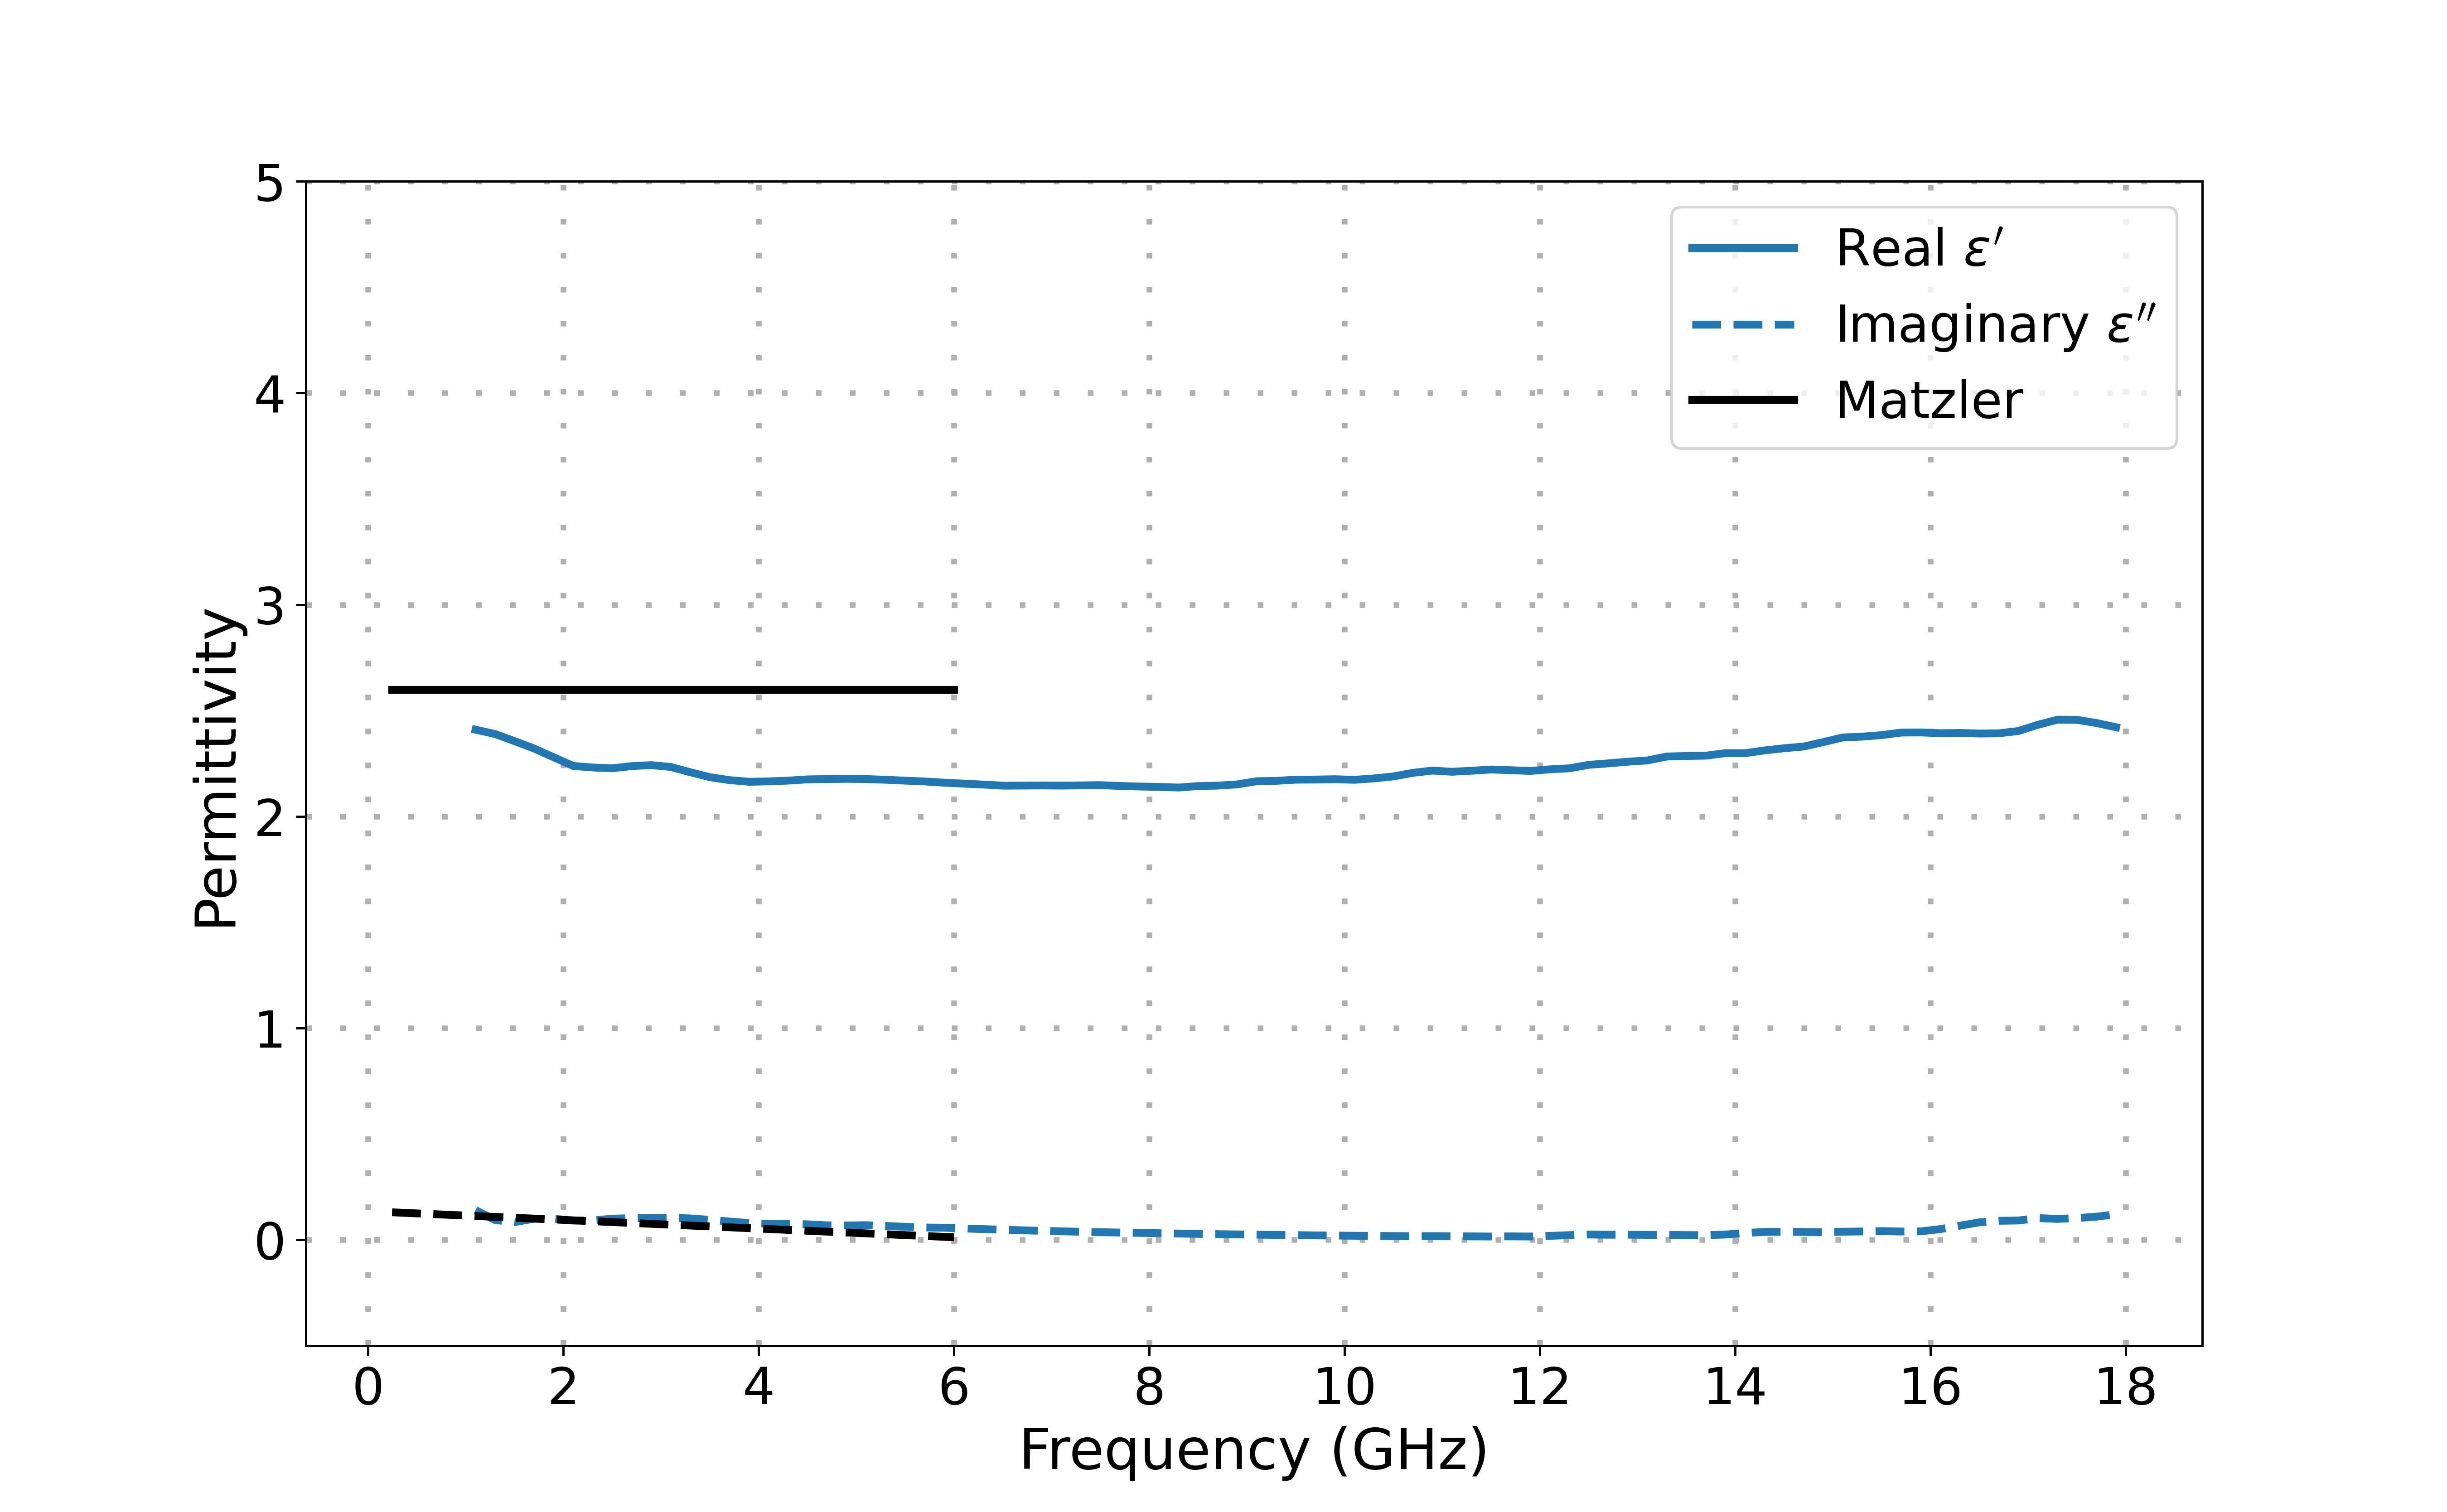
\includegraphics[width=\columnwidth]{Images/dry-sand.png}
    \caption[]{Measurement of dry sand permittivity on all available frequencies compared to the measurements from \textcite{Matzler1998}}\label{fig:dry-sand}
\end{figure}

Figure~\ref{fig:dry-sand} shows that the result obtained from the probe used in the present study are consistent with what was found in the literature with a real permittivity slightly above \(\varepsilon^\prime = 2\) at lower frequencies and around \(\varepsilon^\prime = 2.6\) at the higher end.
However, the permittivity presented in this paper is below the one from \textcite{Matzler1998} in their study range of \qtyrange{0.245}{6}{\giga\hertz}.
This can be explained by the grain size or physical properties of the sand \parencite{Schmugge1980}.
Indeed, varying the density would change the permittivity, where a denser sample would have a higher permittivity since less air (\(\varepsilon^\prime = 1\)) is present in the analyzed volume. 

\subsection{Freezing cycle on wet sand and organic soil}

\begin{figure}[ht!]
    \centering
    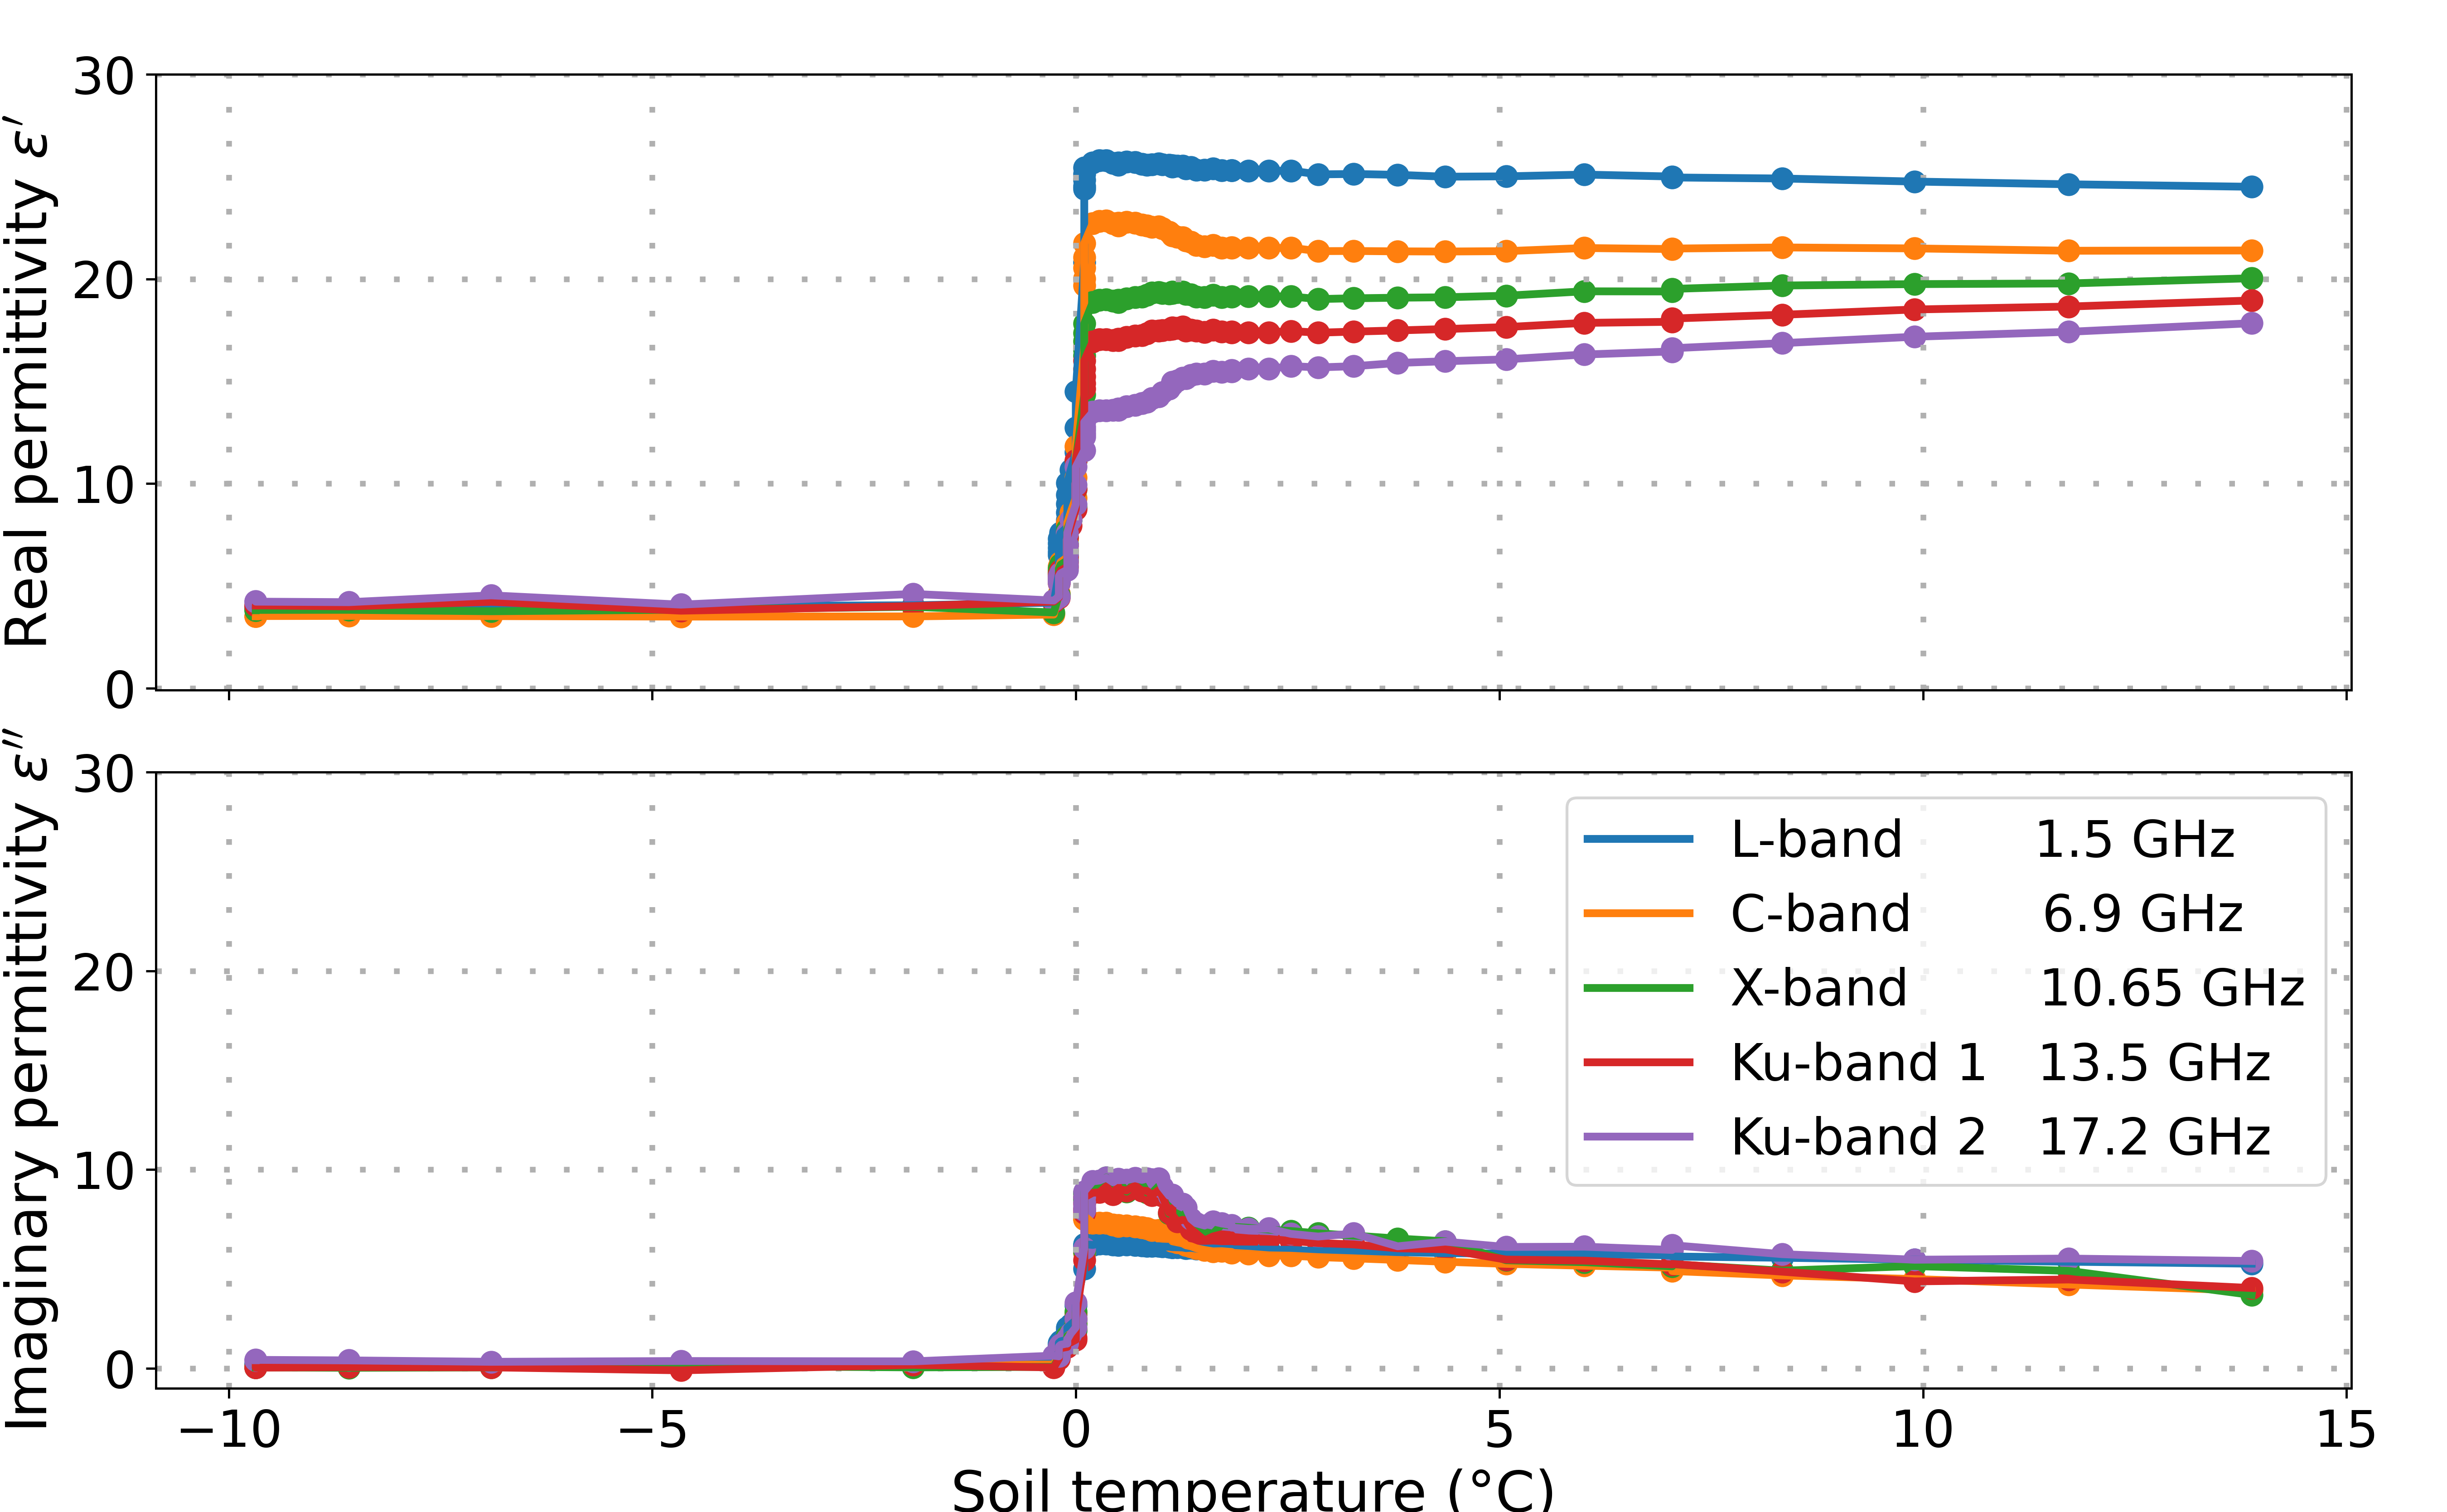
\includegraphics[width=\columnwidth]{Images/wet-sand.png}
    \caption[]{Freeze/thaw cycle of sand with 25\% w/w relative humidity}\label{fig:wet-sand}
\end{figure}

Figure~\ref{fig:wet-sand} shows results of the temperature cycle on the \qty{25}{\percent} weight/weight relative humidity sand.
The graph shows that above \qty{0}{\degreeCelsius}, the permittivity decreases with increasing frequency due to the sand water content, matching what was previously observed for the wet paper (Figure~\ref{fig:wet-paper}).
There also seems to be a slight temperature dependency for the Ku-1- and Ku-2- bands where the permittivity increases as temperature rises.
This increase is due to the variation of the water permittivity as a function of temperature \parencite{Kaatze1989}.
At temperatures lower than \qty{0}{\degreeCelsius}, a sharp decrease in permittivity followed by a plateau is observed, where all frequencies are approximately at the same value (around \(\varepsilon^\prime = 5\)).

\begin{figure}[ht!]
    \centering
    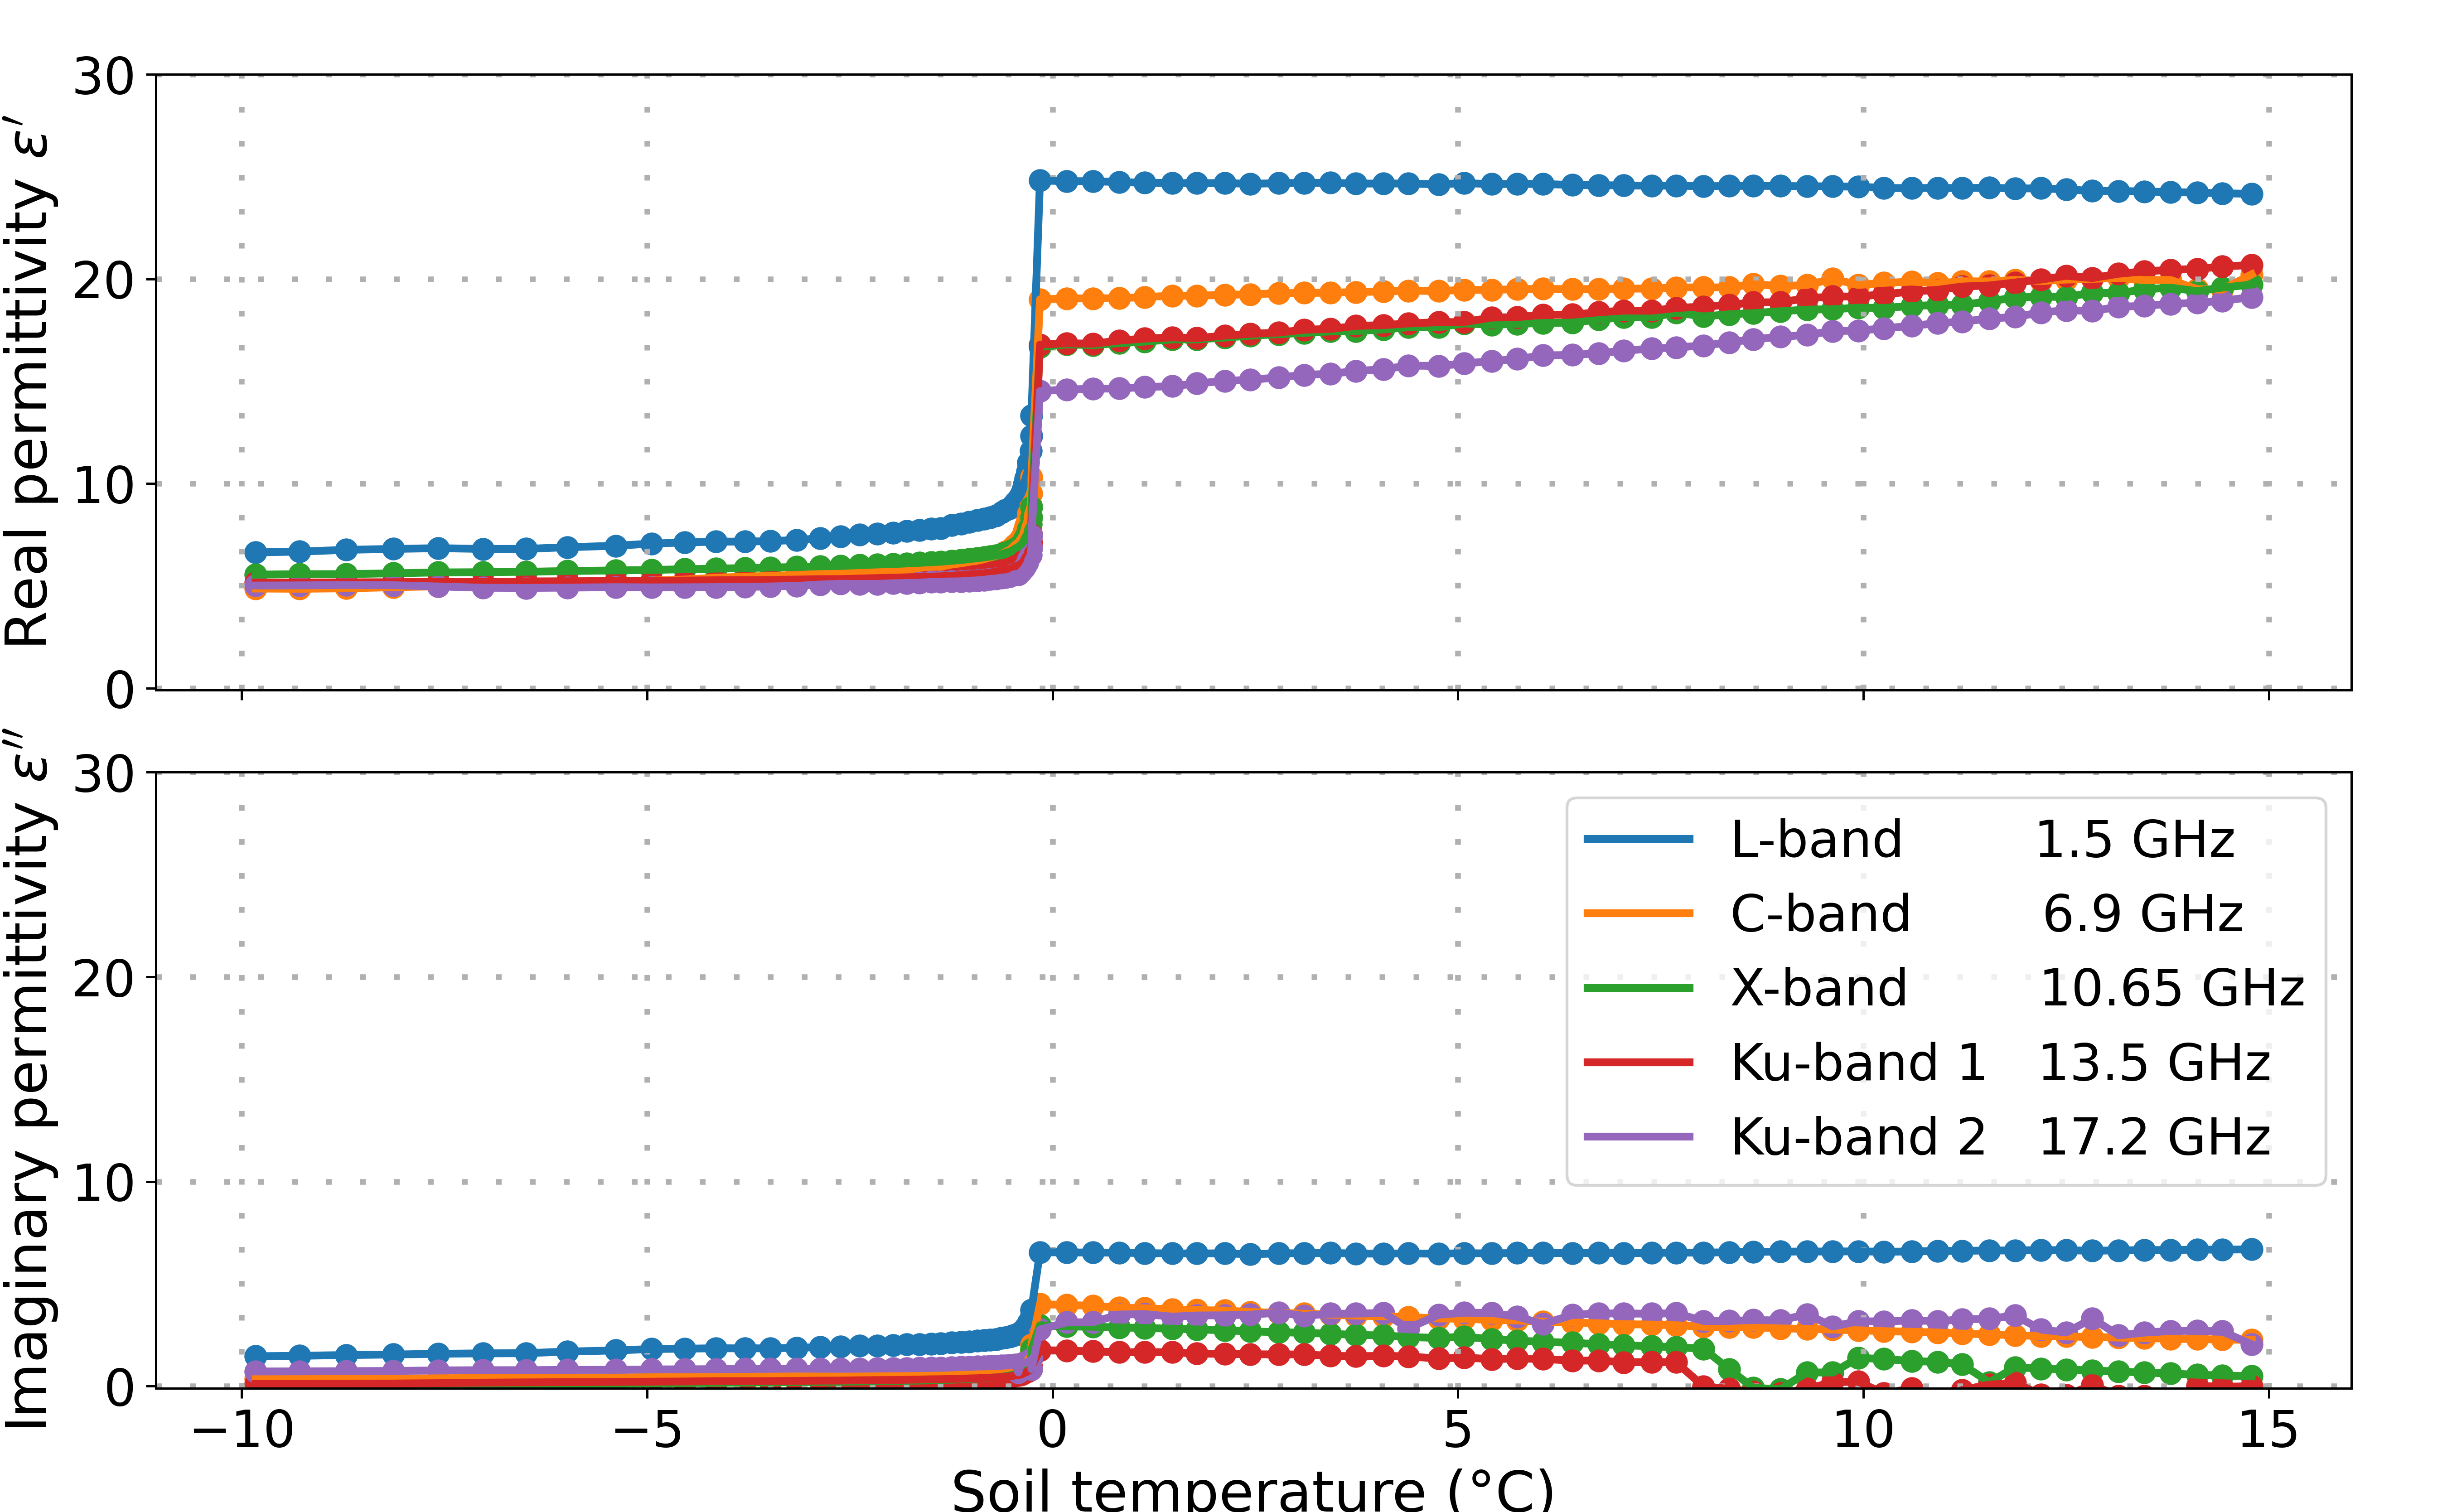
\includegraphics[width=\columnwidth]{Images/wet-soil.png}
    \caption[]{Freeze/thaw cycle of wet organic mesic soil}\label{fig:wet-soil}
\end{figure}

Figure~\ref{fig:wet-soil} shows the permittivity for an arctic organic soil sample (Cambridge Bay).
This sample also seems to show a greater temperature dependency above \qty{0}{\degreeCelsius} for the X- and both Ku-bands than the commercial sand where the permittivity increases with the temperature.
At \qty{15}{\degreeCelsius}, the permittivity of the organic soil sample for the multiple highlighted frequencies converges around \(\varepsilon^\prime = 20\), while the sand sample permittivity is more spread at the same temperature.
The below \qty{0}{\degreeCelsius} permittivity also drops sharply, then plateaus when the water inside the sample is completely frozen at a value around \(\varepsilon^\prime = 5\), like the commercial sand.

Table~\ref{tab:mean-eps} shows the average real permittivity of each plateau when the sample is either completely frozen or completely thawed.
The uncertainty on the numbers presented in the table comes from a standard deviation from the average.
The presented values can be used to parametrize radiative transfer models to compute brightness temperature or backscattering coefficients for remote sensing applications.

\begin{table}[ht!]
\centering
\caption{Mean real permittivity of the frozen (T\(\leq\)\qty{-0.5}{\degreeCelsius}) and thawed (T\(\geq\)\qty{0.5}{\degreeCelsius}) sample for each relevant band frequencies}\label{tab:mean-eps}%
\resizebox{\columnwidth}{!}{%
\begin{tabular}{l c c c c}
    & \multicolumn{2}{c}{Wet sand} & \multicolumn{2}{c}{Organic soil} \\
    & Frozen & Thawed & Frozen & Thawed \\
    \midrule\midrule
    L-band (\SI{1.5}{\giga\hertz})   & \(4.03\pm0.04\) & \(25.3\pm0.2\) &
                                       \(7.6\pm0.6\) & \(24\pm2\) \\
    C-band (\SI{6.9}{\giga\hertz})   & \(3.52\pm0.02\) & \(21.7\pm0.3\) & 
                                       \(5.8\pm0.5\) & \(19\pm2\) \\
    X-band (\SI{10.65}{\giga\hertz}) & \(3.85\pm0.09\) & \(19.2\pm0.2\) & 
                                       \(6.1\pm0.3\) & \(17\pm2\) \\
    Ku-band 1 (\SI{13.5}{\giga\hertz})    & \(4.1\pm0.2\) & \(17.5\pm0.2\) & 
                                            \(5.4\pm0.2\) & \(17\pm2\) \\
    Ku-band 2 (\SI{17.2}{\giga\hertz})    & \(4.3\pm0.2\) & \(15.5\pm0.5\) & 
                                            \(5.1\pm0.2\) & \(15\pm2\) \\
\end{tabular}}
\end{table}

\subsection{Potential applications for satellite missions}
Our unique \acl{oecp} has a large aperture allowing repeatable and precise permittivity measurements of heterogeneous materials while having a frequency band ranging from \qtyrange{0.5}{18}{\giga\hertz}.
The permittivity measurements of the wet commercial sand and of the arctic organic soil sample presented in this work vary greatly whether the soil is frozen or unfrozen, and between the highlighted frequency bands above \qty{0}{\degreeCelsius}.
This has a special importance for \ac{tsmm}, where the soil effect on the snow water equivalent inversion from Ku-band \ac{sar} is still misunderstood \parencite{King2018,Rutter2019}.
Furthermore, at Ku-band, the possible variability of the frozen soil permittivity due to the soil texture and composition, especially for arctic organic soil, is undetermined.
Some studies also show the effect of the zero-curtain \parencite{Outcalt1990,Domine2018} in arctic and boreal forest soils, where the soil under a snowpack is not completely frozen, which can greatly influence the permittivity, hence the backscattering signal.

To follow up this calibration and characterization work with the \ac{oecp}, we plan on applying the freezing/thawing protocol presented above to an array of soil from different places to analyze the permittivity as a function of the soil texture, organic matter percentage, temperature and humidity.
The database created with these soil characterization will then be used to produce a wideband permittivity model spanning the whole probe range.
